% arara: xelatex: {synctex: true}
% arara: indent: {overwrite: yes}
\documentclass[]{IMTexam}

\usepackage[enums]{IMTtikz}

\givecredits
\author{Isabella B.}
\USPN{11810773}
\date{}
\lecture{Física I} % disciplina
\lcode{4302111}
\hwtype{Resolução} % o que é
\examname{Provinha XI} % prova

\begin{document}

\maketitle

\begin{questions}

	\question \label{ques:q1} Considere uma bola de neve que rola \textbf{sem deslizar} em uma ladeira que faz um ângulo $ \theta $ com a horizontal. Durante o percurso, devido à neve depositada na superfície, não só a velocidade, como também a \textbf{massa }da esfera variam no tempo.

	\begin{figure}[H]
		\centering
		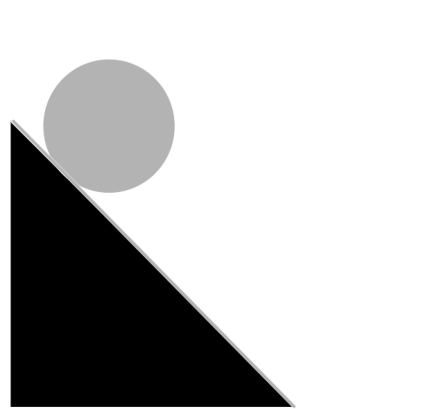
\includegraphics[width=0.5\linewidth]{screenshot001}
		\caption{Representação do problema.}
		\label{fig:fig1}
	\end{figure}

	\begin{parts}
		\part \label{part:q1a} Faça o desenho do diagrama de forças agindo na esfera e escreva as equações de movimento na direção paralela à ladeira.

		\paragraph{Dica:} Lembre-se que a massa da esfera é \textbf{variável}.

		\begin{solution}
			Sabemos que a gravidade $ \vec{g} $ atua na bola de neve, assim como uma força de atrito $ \vec{f} $ (pois ela não desliza), portanto:

			\begin{center}
				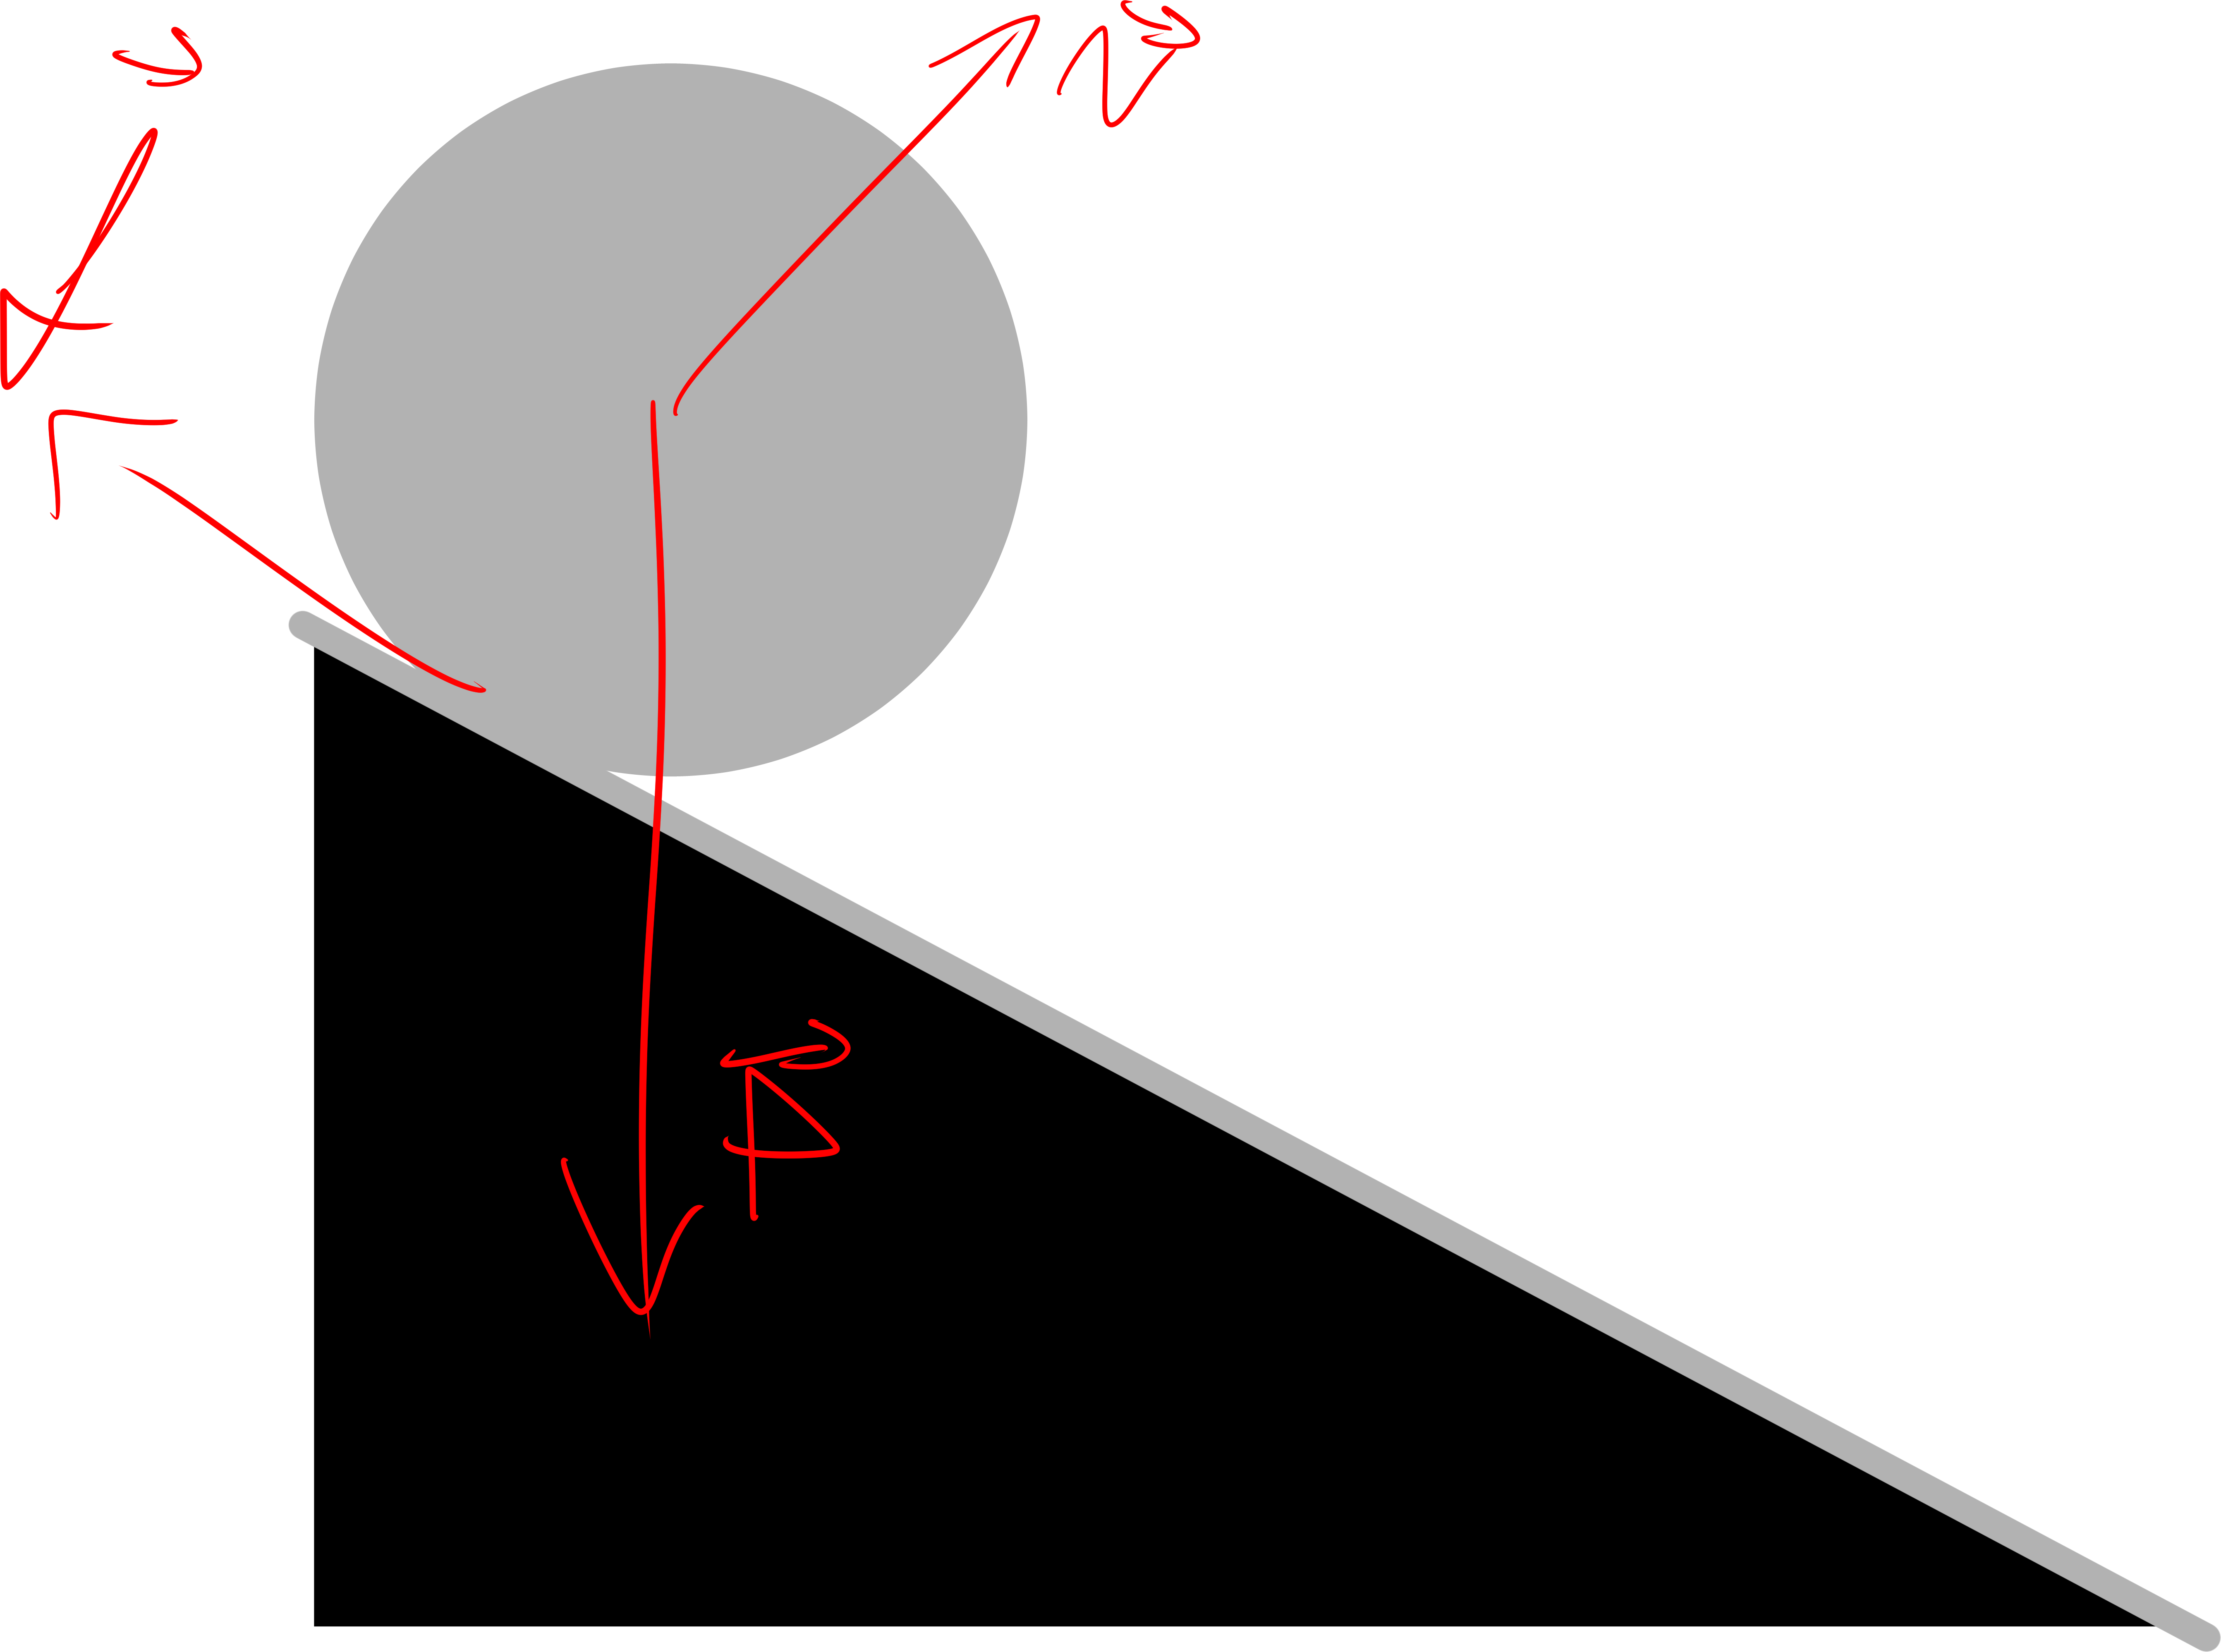
\includegraphics[width=0.5\linewidth]{fig2}
			\end{center}

			Dessa forma, a equação de movimento é
			\begin{equation}\label{eq:eqmov}
				\vec{P}+\vec{N}+\vec{f}=\dod{\vec{p}}{t}
			\end{equation}
			onde $ \vec{p} $ é o momento da bola e $ \vec{P} $ é seu peso.

			Adotando um referencial onde o eixo $ x $ é paralelo ao plano que a bola rola, com o sentido positivo apontado para a descida, e o eixo $ y $ é perpendicular, na direção da normal, positivo para baixo, temos a equação simplificada
			\begin{equation}\label{eq:simp}
				m\,g\sin\theta-f=\dod{\del{m\,v}}{t}
			\end{equation}
			onde $ m $ é a massa em função do tempo, e os módulos dos vetores são denotados por $ |\vec{a}|=a $.
		\end{solution}

		\part \label{part:q1b} Mostre que o momento de inércia de uma esfera rígida que gira ao redor do eixo que passa pelo seu centro é:
		\begin{equation}\label{eq:eq1}
			I=\dfrac{2m\,r^{2}}{5}
		\end{equation}

		\paragraph{Obs:} O resultado pode ser utilizado nos próximos exercícios mesmo que não consiga resolver este item.

		\begin{solution}

			\begin{multi}
				Para encontrar o momento de inércia da situação desejada, podemos considerar infinitos discos com momento de inércia $ \dif I $.

				Pela relação de densidade superficial, temos
				\[ \dif m_d=\dfrac{m_d}{A}\dif A=\dfrac{m_d\,2\pi\,x \dif x}{\pi\,r^{2}}=\dfrac{2m_d\,x\dif x}{\rho^{2}} \]
				onde, $ x $ e $ \rho $ são respectivamente a distância até o eixo de rotação e o raio de um disco à uma altura $ z $ do centro da esfera, e $ m_d $ é a massa do disco.

				Dessa forma, podemos integrar o momento de inércia para um único disco pela relação
				\[ I_d=\int_{0}^{\rho} x^{2}\dif m=\int_{0}^{\rho} \dfrac{2m_d\,x^{3}\dif x}{\rho^{2}}=\dfrac{1}{2}m_d\,\rho^{2}. \]

				\nextcol

				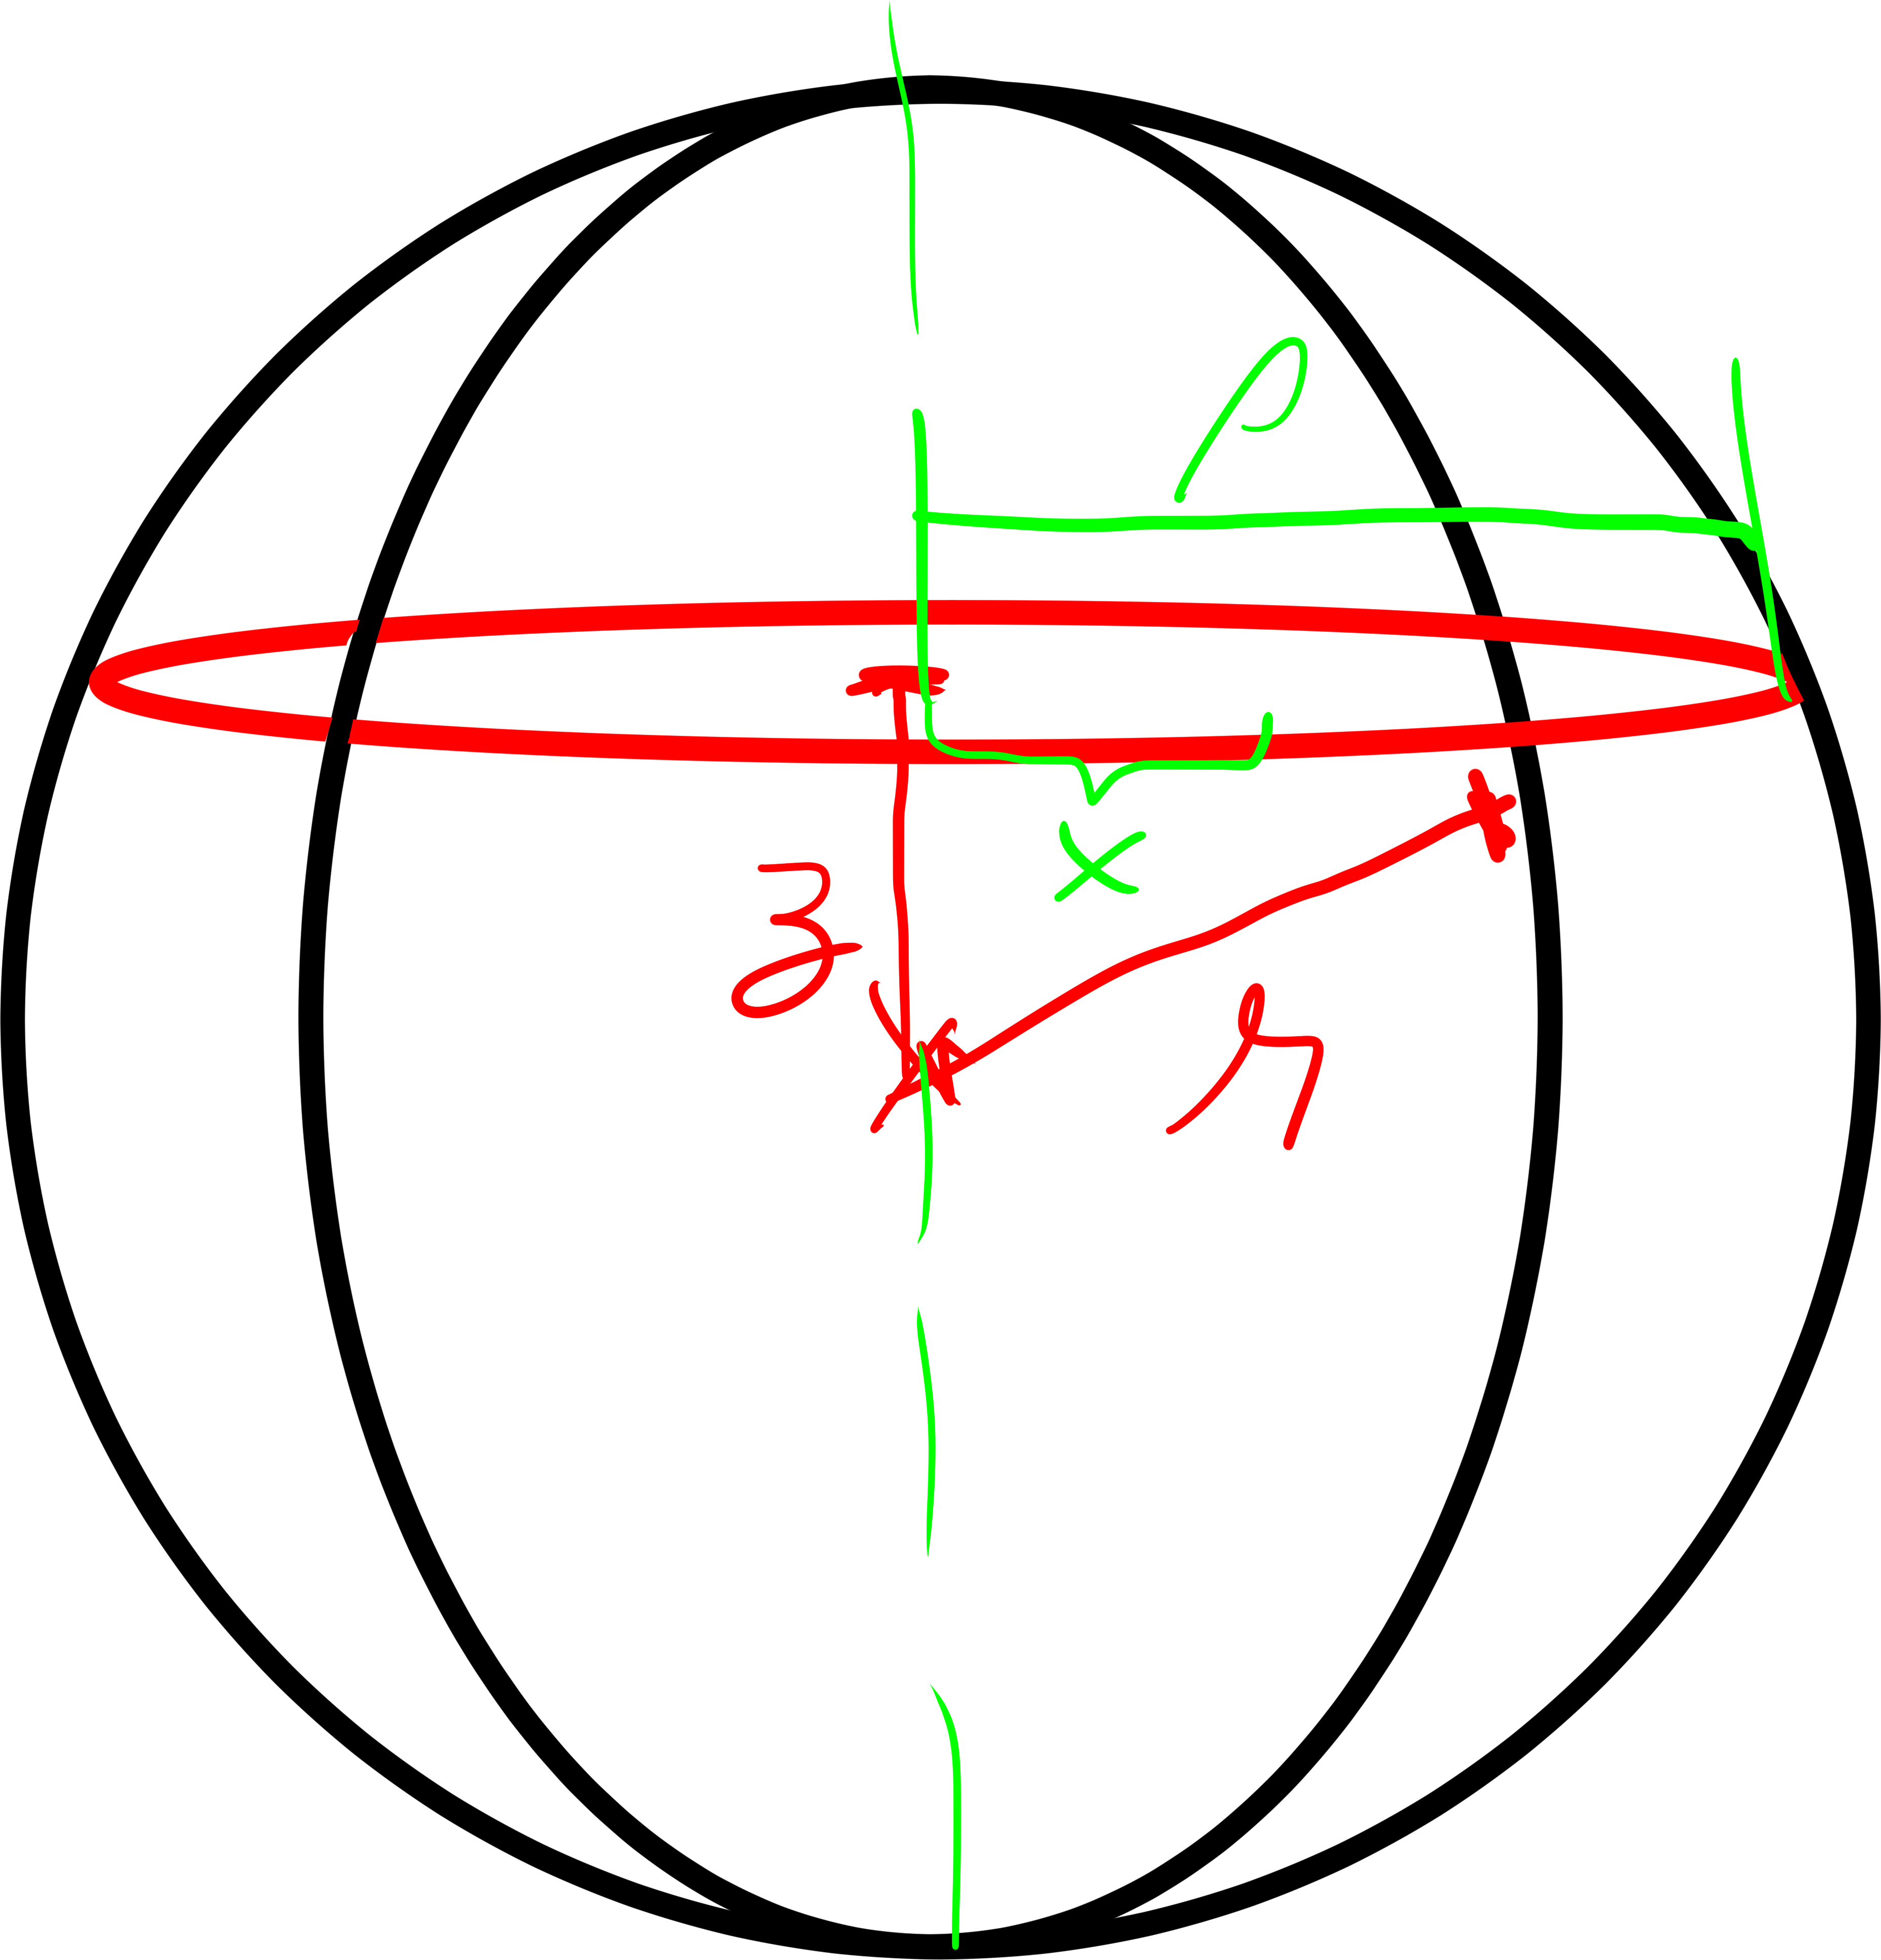
\includegraphics[width=1\linewidth]{fig3}

			\end{multi}


			Portanto, tomando o diferencial $ \dif I=\rho^{2}\dif m/2 $, onde $ \dif m $ é o diferencial de massa da esfera, dado por
			\[ \dif m=\dfrac{m}{V}\dif V=\dfrac{m\,\pi\,\rho^{2}\dif z}{4\pi\,r^{3}/3}=\dfrac{3m\,\rho^{2}\dif z}{4r^{3}} \]

			Por Pitágoras, sabemos que $ \rho^{2}=r^{2}-z^{2} $, portanto
			\[ \dif I=\dfrac{1}{2}\rho^{2}\dfrac{3m\,\rho^{2}\dif z}{4r^{3}}=\dfrac{3m\,\del{r^{2}-z^{2}}^{2}\dif z}{8r^{3}} \]
			e
			\begin{align*}
				I & =\int_{-r}^{r}\dfrac{3m\,\del{r^{4}-2r^{2}\,z^{2}+z^{4}}}{8r^{3}}\dif z           \\
				  & =\eval{\del{\dfrac{3m\,\del{r^{4}\,z-2r^{2}\,z^{3}/3+z^{5}/5}}{8r^{3}}}}_{-r}^{r} \\
				  & =\dfrac{3m\,\del{2r^{5}-4r^{5}/3+2r^{5}/5}}{8r^{3}}                               \\
				  & =\dfrac{3m\,r^{2}\del{30-20+6}}{8\cdot3\cdot5}                                    \\
				I & =\dfrac{2m\,r^{2}}{5}
			\end{align*}
		\end{solution}

		\part \label{part:q1c} Considerando o centro como referência calcule o torque resultante na esfera. Utilize seu resultado para mostrar que a equação de movimento na direção paralela à ladeira pode ser reescrita como:
		\begin{equation}\label{eq:eq2}
			m\,g\sin\theta-\dfrac{I}{r}\dod{\omega}{t}-\dfrac{\omega}{r}\dod{I}{t}=m\dod{v}{t}+v\dod{m}{t}
		\end{equation}

		\begin{solution}
			Sabemos que a força que causa rotação é a força de atrito $ \vec{f} $, sendo o momento angular $ L=I\,\omega $, temos que o módulo do torque $ \vec{\tau} $ é dado por
			\[ \tau=r\,f=\dod{L}{t}=\dod{\del{I\,\omega}}{t}=I\dod{\omega}{t}+\omega\dod{I}{t} \]
			portanto, substituindo em \ref{eq:eqmov}, temos
			\[ P\sin\theta-\del{\dfrac{I}{r}\dod{\omega}{t}+\dfrac{\omega}{r}\dod{I}{t}}=\dod{\del{m\,v}}{t}. \]

			Sendo o peso $ P=m\,g $, aplicando a regra da cadeia no momento, temos
			\[ m\,g\sin\theta-\dfrac{I}{r}\dod{\omega}{t}-\dfrac{\omega}{r}\dod{I}{t}=m\dod{v}{t}+v\dod{m}{t}. \]

			\hfill\qedsymbol
		\end{solution}

		\part \label{part:q1d} Substitua o momento de inércia encontrado em \ref{part:q1b} e utilize o fato de que a esfera rola sem deslizar para reescrever \ref{eq:eq2} como:
		\begin{equation}\label{eq:eq3}
			m\,g\,r\sin\theta-\dfrac{7}{5}v\,r\dod{m}{t}-\dfrac{2}{5}m\,v\dod{r}{t}=\dfrac{7}{5}m\,r\dod{v}{t}
		\end{equation}

		\begin{solution}
			Substituindo \ref{eq:eq2} em \ref{eq:eq3}, temos
			\begin{align*}
				m\,g\sin\theta-\dfrac{\del{2m\,r^{2}/5}}{r}\dod{\omega}{t}-\dfrac{\omega}{r}\dod{\del{2m\,r^{2}/5}}{t}                                                                                           & =m\dod{v}{t}+v\dod{m}{t}            \\
				\intertext{sendo $ \omega=v/r $, temos}
				m\,g\,r\sin\theta-\dfrac{2m\,r^{2}}{5}\dod{\del{v/r}}{t}-\dfrac{v}{r}\del{\dod{m}{t}\dod{}{m}\sbr{\dfrac{2m\,r^{2}}{5}}+\dod{r}{t}\dod{}{r}\sbr{\dfrac{2m\,r^{2}}{5}}}                           & =r\del{m\dod{v}{t}+v\dod{m}{t}}     \\
				m\,g\,r\sin\theta-\dfrac{2m\,r^{2}}{5}\del{\dod{v}{t}\dod{}{v}\sbr{\dfrac{v}{r}}+\dod{r}{t}\dod{}{r}\sbr{\dfrac{v}{r}}}-\dfrac{v}{r}\del{\dod{m}{t}\dfrac{2r^{2}}{5}+\dod{r}{t}\dfrac{4m\,r}{5}} & =r\del{m\dod{v}{t}+v\dod{m}{t}}     \\
				m\,g\,r\sin\theta-\dfrac{2m\,r^{2}}{5}\del{\dod{v}{t}\dfrac{1}{r}-\dod{r}{t}\dfrac{v}{r^{2}}}-v\del{\dod{m}{t}\dfrac{2r}{5}+\dod{r}{t}\dfrac{4m}{5}}                                             & =r\del{m\dod{v}{t}+v\dod{m}{t}}     \\
				m\,g\,r\sin\theta-v\,r\dod{m}{t}\del{1+\dfrac{2}{5}}-m\,v\dod{r}{t}\del{\dfrac{4}{5}-\dfrac{2}{5}}                                                                                               & =m\,r\dod{v}{t}\del{1+\dfrac{2}{5}} \\
				m\,g\,r\sin\theta-\dfrac{7}{5}v\,r\dod{m}{t}-\dfrac{2}{5}m\,v\dod{r}{t}                                                                                                                          & =\dfrac{7}{5}m\,r\dod{v}{t}
			\end{align*}
		\end{solution}

		\part \label{part:q1e} Assumindo que a densidade $ \rho $ da esfera seja constante. Encontre a taxa de variação da massa com o raio $ \od{m}{r} $. Substitua em \ref{eq:eq3} e mostre que a equação se torna:
		\begin{equation}\label{eq:eq4}
			g\,r\sin\theta-\dfrac{23}{5}v\dod{r}{t}=\dfrac{7}{5}r\dod{v}{t}
		\end{equation}

		\begin{solution}
			Pela relação da densidade, temos
			\begin{align}
				m          & =\rho\,V=\rho\,\dfrac{4}{3}\pi\,r^{3}\nonumber                       \\
				\intertext{derivando com respeito ao raio}
				\dod{m}{r} & =\rho\,4\pi\,r^{2}\nonumber                                          \\
				\dod{m}{r} & =\dfrac{m}{4\pi\,r^{3}/3}\,4\pi\,r^{2}=\dfrac{3m}{r}.\label{eq:rhod}
			\end{align}
			Retomando \ref{eq:eq4}
			\begin{align*}
				g\,r\sin\theta-\dfrac{1}{m}\dfrac{7}{5}v\,r\dod{m}{r}\dod{r}{t}-\dfrac{2}{5}v\dod{r}{t} & =\dfrac{7}{5}r\dod{v}{t}  \\
				\intertext{substituindo \ref{eq:rhod}}
				g\,r\sin\theta-\del{\dfrac{1}{m}\dfrac{7}{5}r\,\dfrac{3m}{r}+\dfrac{2}{5}}v\dod{r}{t}   & =\dfrac{7}{5}r\dod{v}{t}  \\
				g\,r\sin\theta-\dfrac{23}{5}v\dod{r}{t}                                                 & =\dfrac{7}{5}r\dod{v}{t}.
			\end{align*}

			\hfill\qedsymbol
		\end{solution}

		\part \label{part:q1f} Assumindo que o raio aumenta no tempo à uma taxa constante por rotação da esfera:
		\begin{equation}\label{eq:eq5}
			\dod{r}{t}=\dfrac{k}{2\pi/\omega}=\dfrac{k\,v}{2\pi\,r}
		\end{equation}

		A equação \ref{eq:eq4} pode ser escrita como:
		\begin{equation}\label{eq:eq6}
			g\sin\theta-\dfrac{23v^{2}\,k}{10\pi\,r^{2}}=\dfrac{7}{5}\dod{v}{t}
		\end{equation}

		Essa equação diferencial não pode ser resolvida analiticamente%
		\footnote{É possível reescrever a equação de forma a achar a velocidade e aceleração como funções do raio. Nesse caso existe solução analítica.}.
		Porém podemos estudar o comportamento da aceleração da bola de neve tomando a derivada de \ref{eq:eq6} em relação ao tempo. Feito isso, encontre a aceleração terminal em termos de $ g $ e $ \theta $.

		\begin{solution}
			Derivando \ref{eq:eq6} com relação ao tempo, temos
			\begin{align*}
				\dod{}{t}\sbr{g\sin\theta-\dfrac{23v^{2}\,k}{10\pi\,r^{2}}}                                                                        & =\dod{}{t}\sbr{\dfrac{7}{5}\dod{v}{t}}                           \\
				g\cos\theta-\dfrac{23k}{10\pi}\dod{}{t}\sbr{\del{\dfrac{v}{r}}^{2}}                                                                & =\dfrac{7}{5}\dod[2]{v}{t}                                       \\
				g\cos\theta-\dfrac{23k}{10\pi}\del{2\dfrac{v}{r}\del{\dod{v}{t}\dod{}{v}\sbr{\dfrac{v}{r}}+\dod{r}{t}\dod{}{r}\sbr{\dfrac{v}{r}}}} & =\dfrac{7}{5}\dod[2]{v}{t}                                       \\
				g\cos\theta-\dfrac{23k}{5\pi}\dfrac{v}{r}\del{\dfrac{1}{r}\dod{v}{t}-\dfrac{k\,v}{2\pi\,r}\dfrac{1}{r^{2}}}                        & =\dfrac{7}{5}\dod[2]{v}{t}                                       \\
				\intertext{a aceleração terminal se dá quando ela não varia mais, portanto, $ \od[2]{v}{t}=0 $}
				g\cos\theta-\dfrac{23k\,v}{5\pi\,r}\del{\dod{v}{t}-\dfrac{k\,v}{2\pi\,r^{2}}}                                                      & =0                                                               \\
				\dfrac{23k\,v}{5\pi\,r}\dod{v}{t}                                                                                                  & =g\cos\theta+\dfrac{23k\,v}{5\pi\,r}\dfrac{k\,v}{2\pi\,r^{2}}    \\
				\Aboxed{\dod{v}{t}                                                                                                                 & =\dfrac{5\pi\,g\,r}{23k\,v}\cos\theta+\dfrac{k\,v}{2\pi\,r^{2}}}
			\end{align*}
		\end{solution}
	\end{parts}


\end{questions}
\end{document}
